%# -*- coding: utf-8-unix -*-
%%==================================================
%% chapter01.tex for SJTU Master Thesis
%%==================================================

%\bibliographystyle{sjtu2}%[此处用于每章都生产参考文献]
\chapter{系统实现}
\label{chap:sys_implement}

上一章介绍了系统的设计,这一章将首先介绍系统实现所需的预备知识,进而介绍系统的具体实现。

\section{预备知识}

由于系统位于linux内核态,因此需要对内核中与系统实现相关的基本知识进行介绍。这些预备知识包括Linux存储层次、bio、Device Mapper等。

\subsection{Linux存储层次}

Linux存储层次如图\ref{fig:linux_storage_layer}所示,大致可分为共六层\cite{敖青云2011存储技术原理分析}:

\begin{enumerate}
    \item 最上层位于用户态,对用户看到的文件,用户的应用程序通过调用POSIX接口对这些文件进行操作。

    \item 第二层为虚拟文件系统(VFS, virtual file system)层,位于内核态。VFS的作用为屏蔽其所管理的具体文件系统,使用户可以使用统一的接口进行调用。POSIX在VFS层将数据封装成bio,然后将bio交给挂载的具体文件系统执行操作,bio将在\ref{sec:bio}具体介绍。

    \item 第三层为块层(block layer),位于内核态。块层负责将bio封装成设备请求(request)。具体封装方法为:如果几个bio的读写区域连续,那么将他们积攒成一个request,request下挂多个连续bio,即合并bio请求。如果bio跟其它bio都不连续,则它自己创建一个新request,将自己挂到这个request下。每个request下能挂的bio有限,多个连续bio的访问总区域超过一定限额,就不能合并为一个request。之所以不将多个bio合并为一个bio而是使用request,是因为每个bio都有自己的回调,如果合并为一个bio则失去了对不同bio使用不同回调的灵活性。合并后的request会以队列的形式组织起来,等待SCSI层进行处理。

    \item 第四层为SCSI层,位于内核态。SCSI层负责将request封装成与块设备具体存储格式相关的SCSI命令。

    \item 第五层为设备驱动(device driver)层,位于内核态,负责接收SCSI命令,并将其转换为设备请求,将其放入设备请求队列。

    \item 第六层为具体的设备层,位于内核态,负责接收设备请求,并在实际设备上执行对应的操作。

\end{enumerate}

\begin{figure}[!htp]
    \centering
    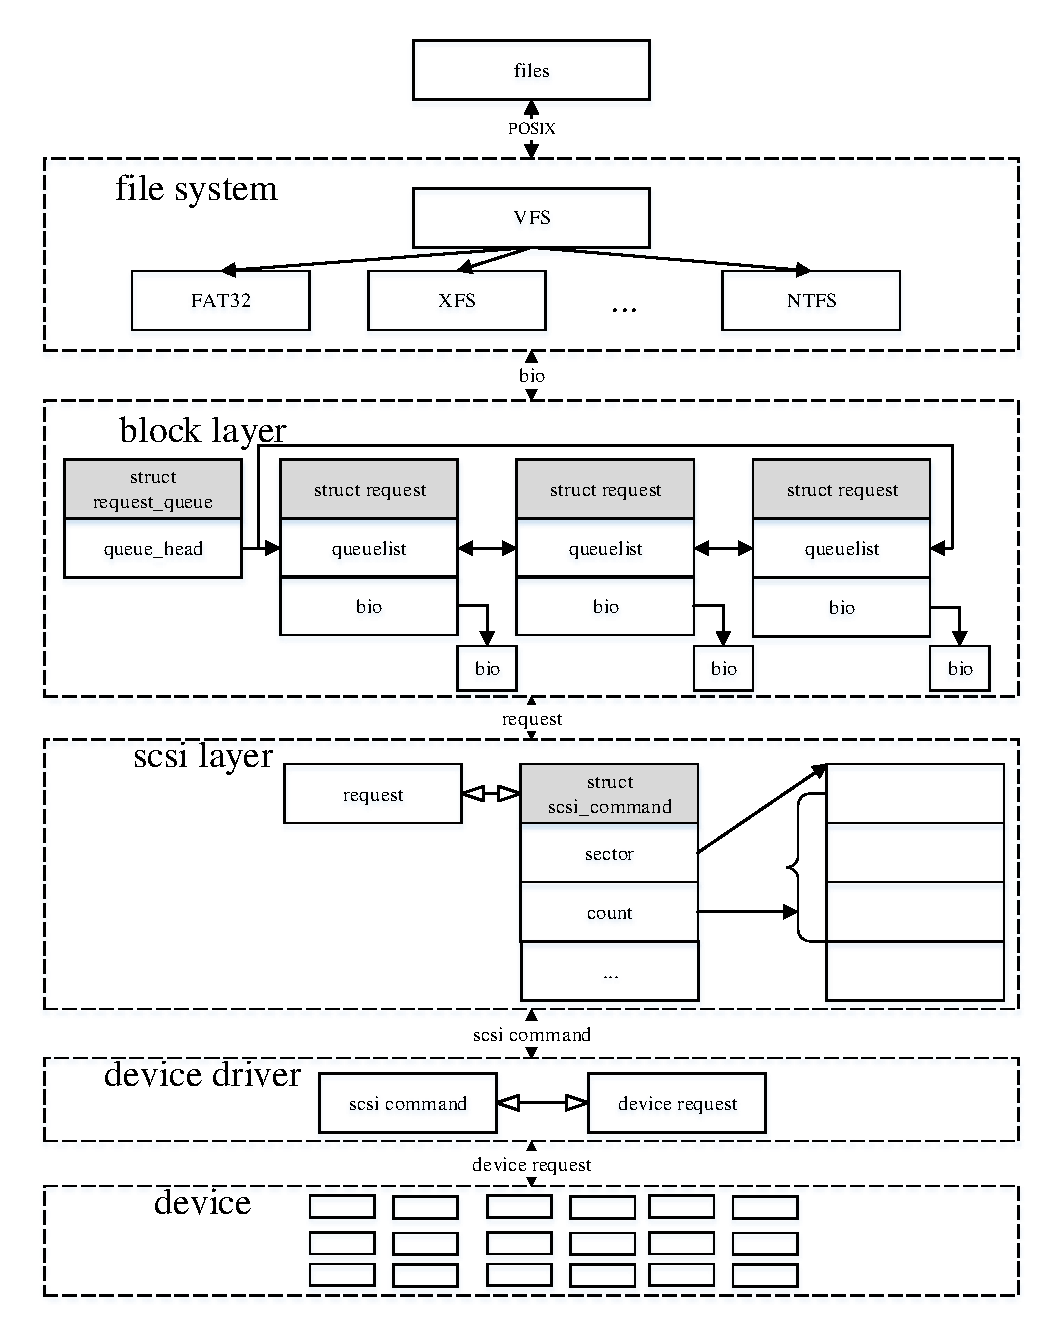
\includegraphics[width=\textwidth]{linux_storage_layer.pdf}
    \bicaption[fig:linux_storage_layer]{Linux存储层次}{Linux存储层次}{Fig}{linux storage layer}
\end{figure}

\subsection{bio}
\label{sec:bio}

bio这一数据结构被用来描述块设备的I/O操作,将内存缓冲区与块设备联系起来的重要桥梁\cite{corbet2005linux}。

bio的具体结构如图\ref{fig:bio}所示。一个bio指针指向由bio结构体组成的链表,bio结构体中的bi\_io\_vec指向一个bi\_vec结构体数组,每个bi\_vec结构体中bv\_page指向内存中的实际页,bv\_offset和bv\_len组合来定位数据在该页中的具体位置,如此,一个bio链表就将散落在内存中的各数据组织为一个块设备请求。

\begin{figure}[!htp]
    \centering
    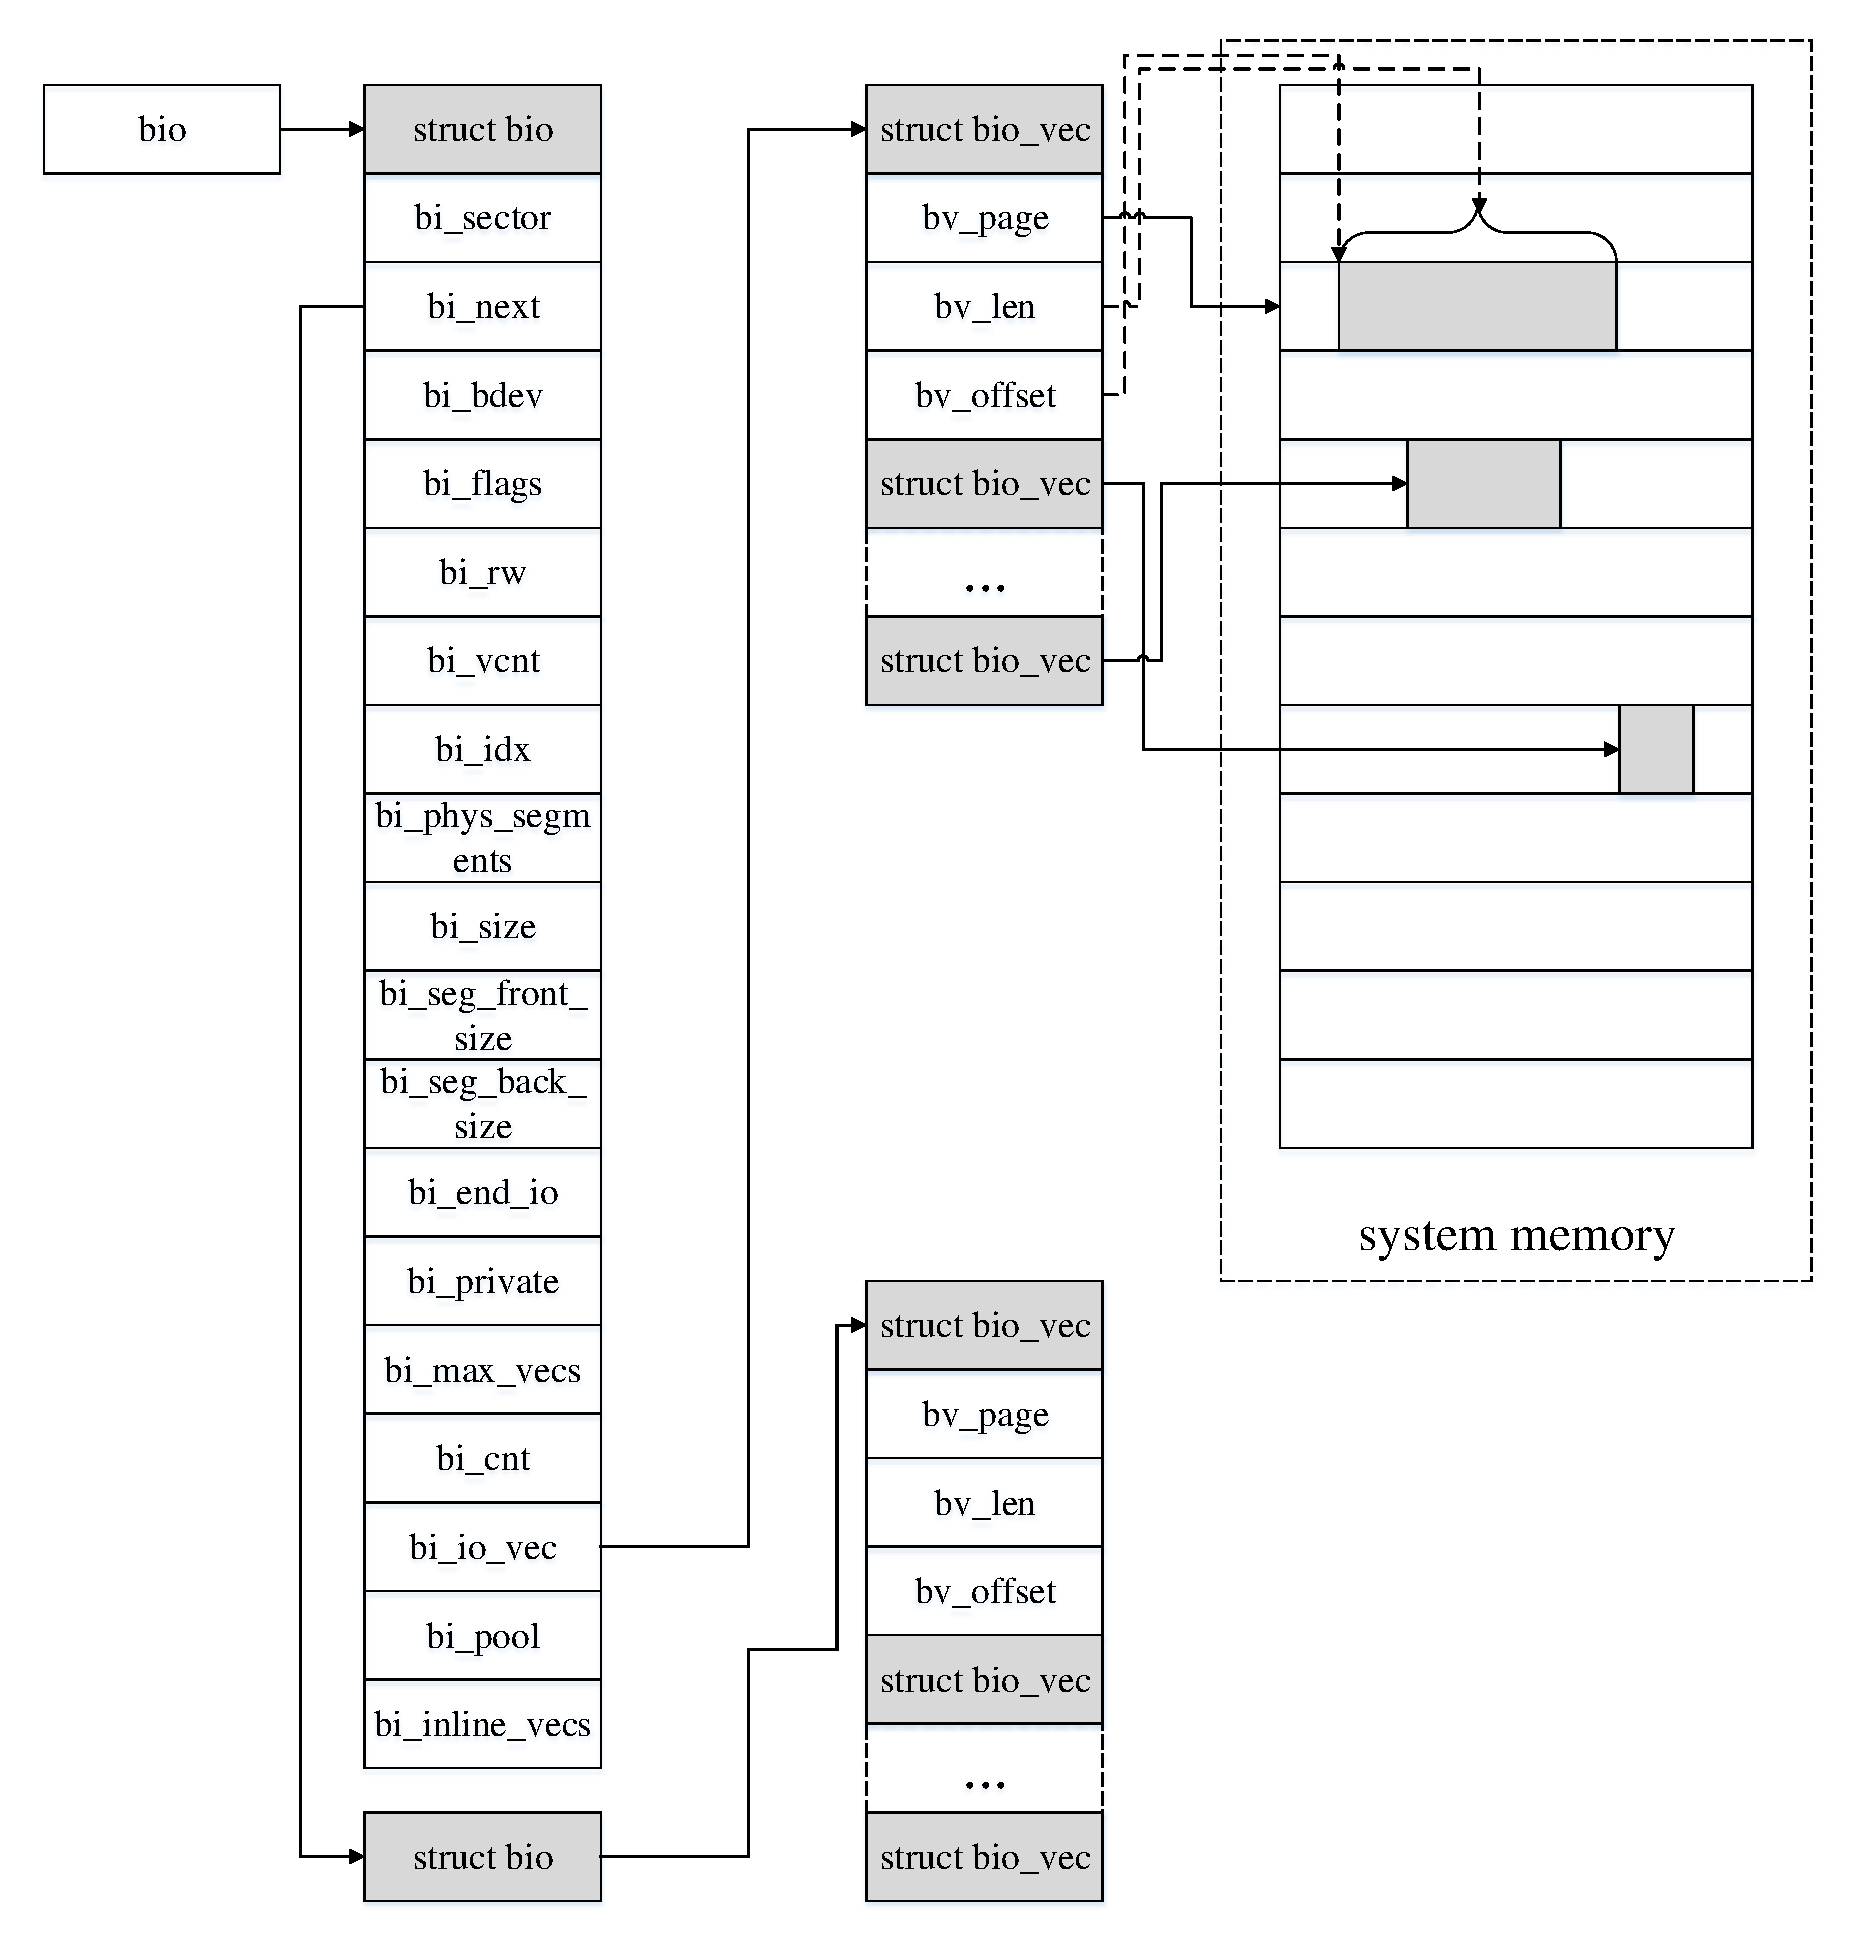
\includegraphics[width=0.8\textwidth]{bio.pdf}
    \bicaption[fig:bio]{bio结构}{bio结构}{Fig}{bio structure}
\end{figure}

\subsection{Device Mapper}

Device Mapper是Linux2.6 内核中支持逻辑卷管理的通用设备映射机制,它为实现用于存储资源管理的块设备驱动提供了一个高度模块化的内核架构\cite{bovet2005understanding}。Device Mapper以一个块设备驱动在内核中注册,它包含mapped device、mapping table、target device这三个重要概念。mapped device可以理解为内核对外提供的逻辑设备,用户看到的也是这个逻辑设备,mapped device通过mapping table组织与与target device的映射关系,一个mapped device可以映射到一个或者多个target device上,总体层次如图\ref{fig:device_mapper}所示,target device可以是真实的物理设备也可以是另一个mapped device,如此迭代,形成一个树状结构。

\begin{figure}[!htp]
    \centering
    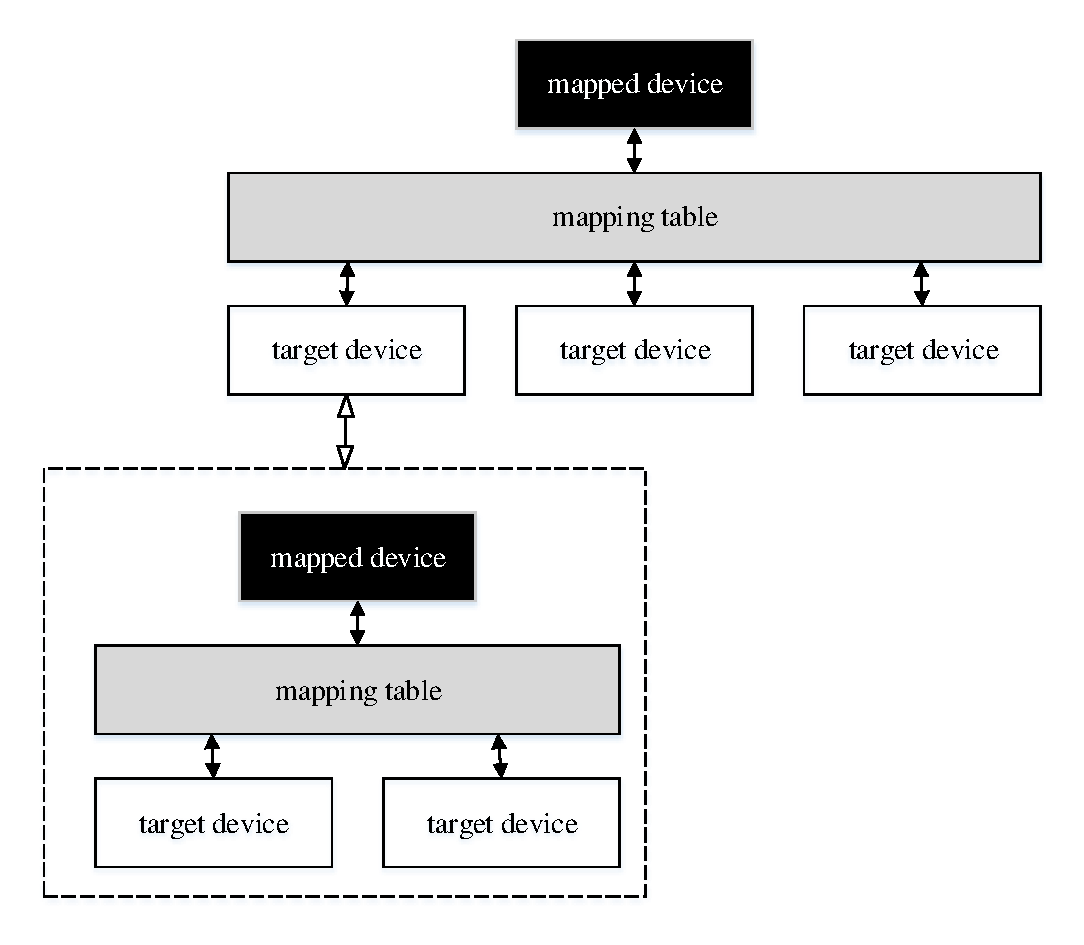
\includegraphics[width=0.8\textwidth]{device_mapper.pdf}
    \bicaption[fig:device_mapper]{Device Mapper层次图}{Device Mapper层次图}{Fig}{Device Mapper Layer}
\end{figure}

Device Mapper的实现原理是将mapped device的make\_request\_fn方法实现为自己的dm\_request,这个经过mapped device的bio请求都会进入dm\_request方法,之后Device Mapper通过判断mapped device是基于request还是基于bio来分别处理:

如果mapped device是基于request的,那么和磁盘设备一样通过generic\_make\_request把bio合并为request,将其放到mapped device的request队列中,当mapped device通过kblockd调用dm\_request\_fn时,dm\_request\_fn中会调用peek\_request从mapped device的request队列中拿出request将其clone(clone生成的request中的bio与原request中的bio指向同一个内存页,clone操作只是分配新的bio和request),然后通过调用map\_request将request映射,将clone后的request发往低层的真实设备。

如果mapped device是基于bio的,那么调用\_dm\_request首先clone bio然后调用\_\_map\_bio将bio映射,将clone后的bio通过generic\_make\_request发往低层的真实设备。

mapped device基于request还是基于bio的主要区别在于,如果是基于request则request是放在mapped device的request队列中,如果是基于bio,则是在调用generic\_make\_request总将bio封装成request放到真实设备的request队列中。


\subsection{其他预备知识}

在系统的实现过程中,除了上面介绍的几个关键知识点外,还涉及很多其他的Linux内核知识,比如Linux的内核模块编程、内核编程中的常用宏、常用数据结构、内核的调试等内容,这里不再详细介绍。

\section{编程实现}

有了上面预备知识的铺垫,就可以比较清楚地介绍系统的编程实现了。下面将着重介绍系统的对多缓存设备对多后台设备的实现以及按照进程的权限分配不同进程的I/O带宽的实现。本系统基于的内核版本为linux 3.10.108。

\subsection{多缓存设备对多后台设备的实现}

在设计部分提过本系统采用分层管理结构,将多设备的管理与混合存储系统隔离开。本系统对多缓存设备对多后台设备的实现基于LVM。系统的建立流程如图\ref{fig:create}所示,首先接收用户的各种参数信息,然后依据参数先将多个SSD映射为一个虚拟缓存设备,再将多个HDD映射为一个虚拟后台设备,最后将这两个设备的信息连同混合存储系统的配置参数发给dmsetup命令,dmsetup将参数传给系统在内核的初始化函数进行混合存储系统的构建。系统的销毁流程比较简单,首先调用系统在内核的注销函数销毁混合存储系统,然后将虚拟缓存设备卸载解除与多个SSD的映射关系,再将虚拟后台设备卸载解除与多个HDD的映射关系。

\begin{figure}[!htp]
    \centering
    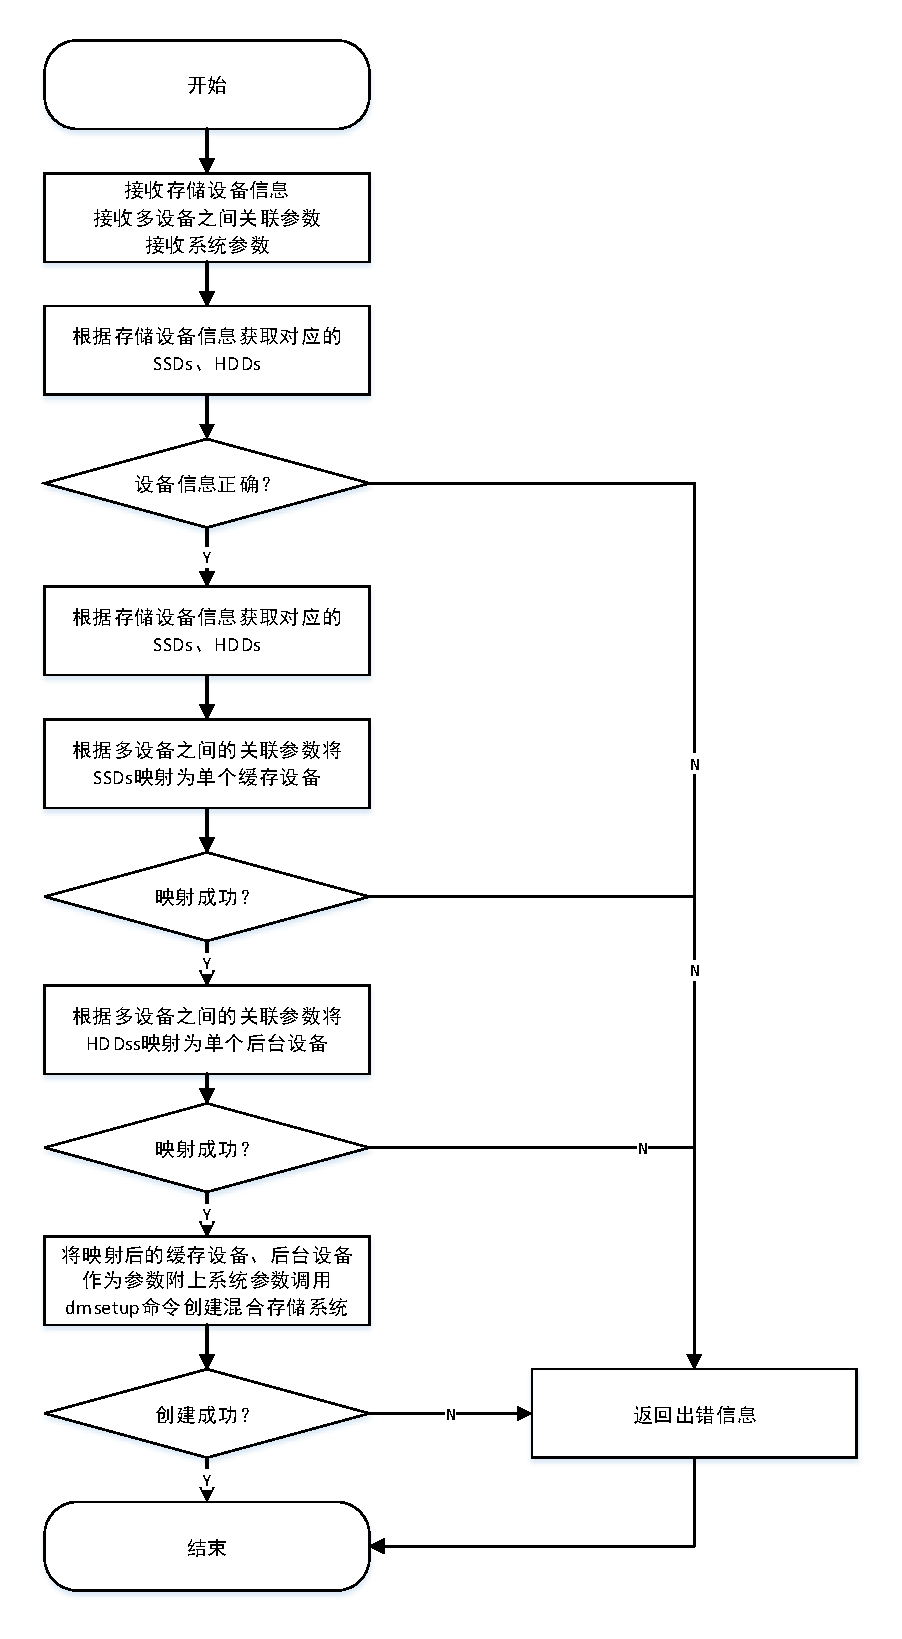
\includegraphics[width=0.6\textwidth]{create.pdf}
    \bicaption[fig:create]{多缓存设备对多后台设备的创建}{多缓存设备对多后台设备的创建}{Fig}{creation of multi-ssds to multi-hdds}
\end{figure}

\subsection{按照进程的权限分配不同进程的I/O带宽的实现}

本系统通过使用Linux自带的I/O调度器的CFQ策略,通过为不同进程设置不同的cgroup的weight实现对这些进程按照权重不同分配不同的I/O带宽。由于I/O调度器只对request队列起作用,对bio不起作用,因此需要实现基于request的混合存储系统。

\subsubsection{Linux内核的修改}

通过研究Linux内核中Device Mapper的相关代码,本研究发现现有的Device Mapper的实现中,仅有multipath\_map函数是基于request的,在multipath\_map可以改变request队列然后返回DM\_MAPIO\_REMAPPED达成对队列的修改,而负责将对mapped device的请求映射到低层的设备的函数map\_rq必须将请求发送给低层设备而不能仅改变队列就返回。因此需要实现一个新的接口。Device Mapper提供了target\_type这一结构体用来管理对mapped device的各种操作,在target\_type中添加mk\_rq接口实现对request的生成。

对Linux的内核作出的具体修改如下:

\begin{enumerate}
    \item include/linux/dm-io.h文件对dm\_io\_request结构体添加三个变量,submit\_bio用以表示是否直接提交bio,start和end为两个bio指针,指向该dm\_io\_request的起始bio和终止bio。
    \item drivers/md/dm-io.c文件,do\_region改为接收dm\_io\_request类型参数,依据dm\_io\_request类型的参数中submit\_bio的设置判断是直接提交bio还是放入request中。dispatch\_io改为接收dm\_io\_request类型参数,相关操作包括对do\_region的调用相应改为基于dm\_io\_request类型的操作。sync\_io改为接收dm\_io\_request类型参数,相关操作包括对dispatch\_io的调用相应改为基于dm\_io\_request类型的操作。async\_io改为接收dm\_io\_request类型参数,相关操作包括对dispatch\_io的调用相应改为基于dm\_io\_request类型的操作。dm\_io中对sync\_io和async\_io的调用都改为传递dm\_io\_request类型参数。
    \item include/linux/device-mapper.h文件中对target\_type结构体添加函数指针mk\_rq作为新的新接口,用以支持自己对request的生成。
    \item drivers/md/dm.c文件,dm\_request原本只是简单地判断mapped device是基于request还是基于bio,并据此分别调用blk\_queue\_bio或\_dm\_request。现在首先从映射表中获得mapped device,查看是否实现了具体的mk\_rq方法,如果实现了则调用该方法然后返回,否则依旧根据是基于request还是基于bio分别调用blk\_queue\_bio或\_dm\_request,流程如图\ref{fig:dm_request}所示。
    \item drivers/md/dm-bufio.c文件,use\_dmio和dm\_bufio\_issue\_flush中初始化io\_req时设置submit\_bio为1,默认直接提交bio。
    \item drivers/md/dm-kcopyd.c文件,run\_io\_job中初始化io\_req时设置submit\_bio为1,默认直接提交bio。
    \item drivers/md/dm-log.c文件,create\_log\_context中设置lc的io\_req的submit\_bio为1,默认直接提交bio。
    \item drivers/md/dm-raid1.c文件,mirror\_flush、read\_async\_bio和do\_write中初始化io\_req时设置submit\_bio为1,默认直接提交bio。
    \item drivers/md/dm-snap-persistent.c文件,chunk\_io中初始化io\_req时设置submit\_bio为1,默认直接提交bio。
\end{enumerate}

\begin{figure}[!htp]
    \centering
    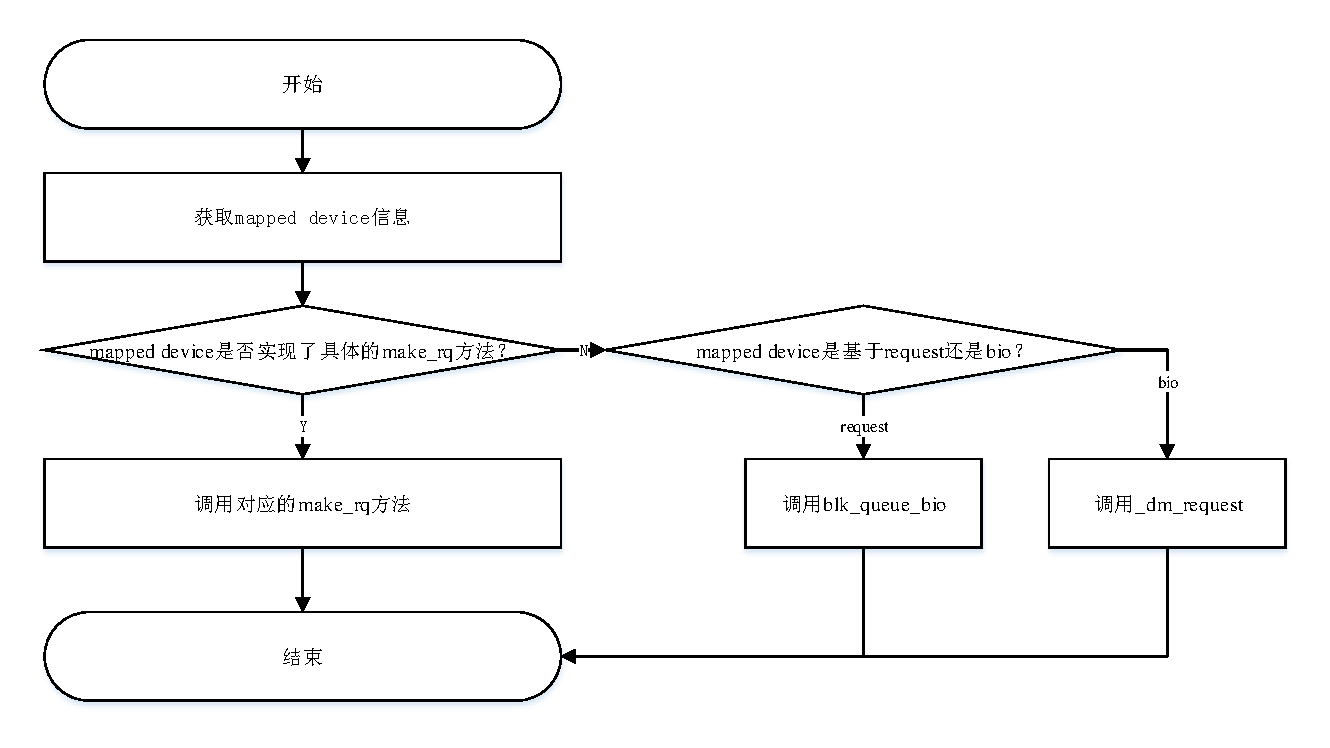
\includegraphics[width=\textwidth]{dm_request.pdf}
    \bicaption[fig:dm_request]{dm\_request处理流程}{dm\_request处理流程}{Fig}{dm\_request process}
\end{figure}


\subsubsection{系统的实现}

在对Linux内核修改完毕后,现在的Device Mapper中target\_type支持开发者实现自己的mk\_rq接口。本系统通过实现mk\_rq和map\_rq接口实现基于request的混合存储系统,具体流程如图\ref{fig:request_process}所示。

mk\_rq()负责用bio生成对应的request,mk\_rq()接收对系统的bio请求,然后根据bio判断对系统的具体操作,然后去调用对应操作的函数并传入参数设置不立即提交bio,各操作函数经过递归调用最后都会落到dm\_io\_async\_bvec()中,m\_io\_async\_bvec()根据传入的参数生成dm\_io\_request并根据最初的参数判断不是立即提交bio,于是将bio存入mapped device的request队列中。

map\_rq()负责将对混合存储系统的请求分派到具体的实际设备执行操作。

\begin{figure}[!htp]
    \centering
    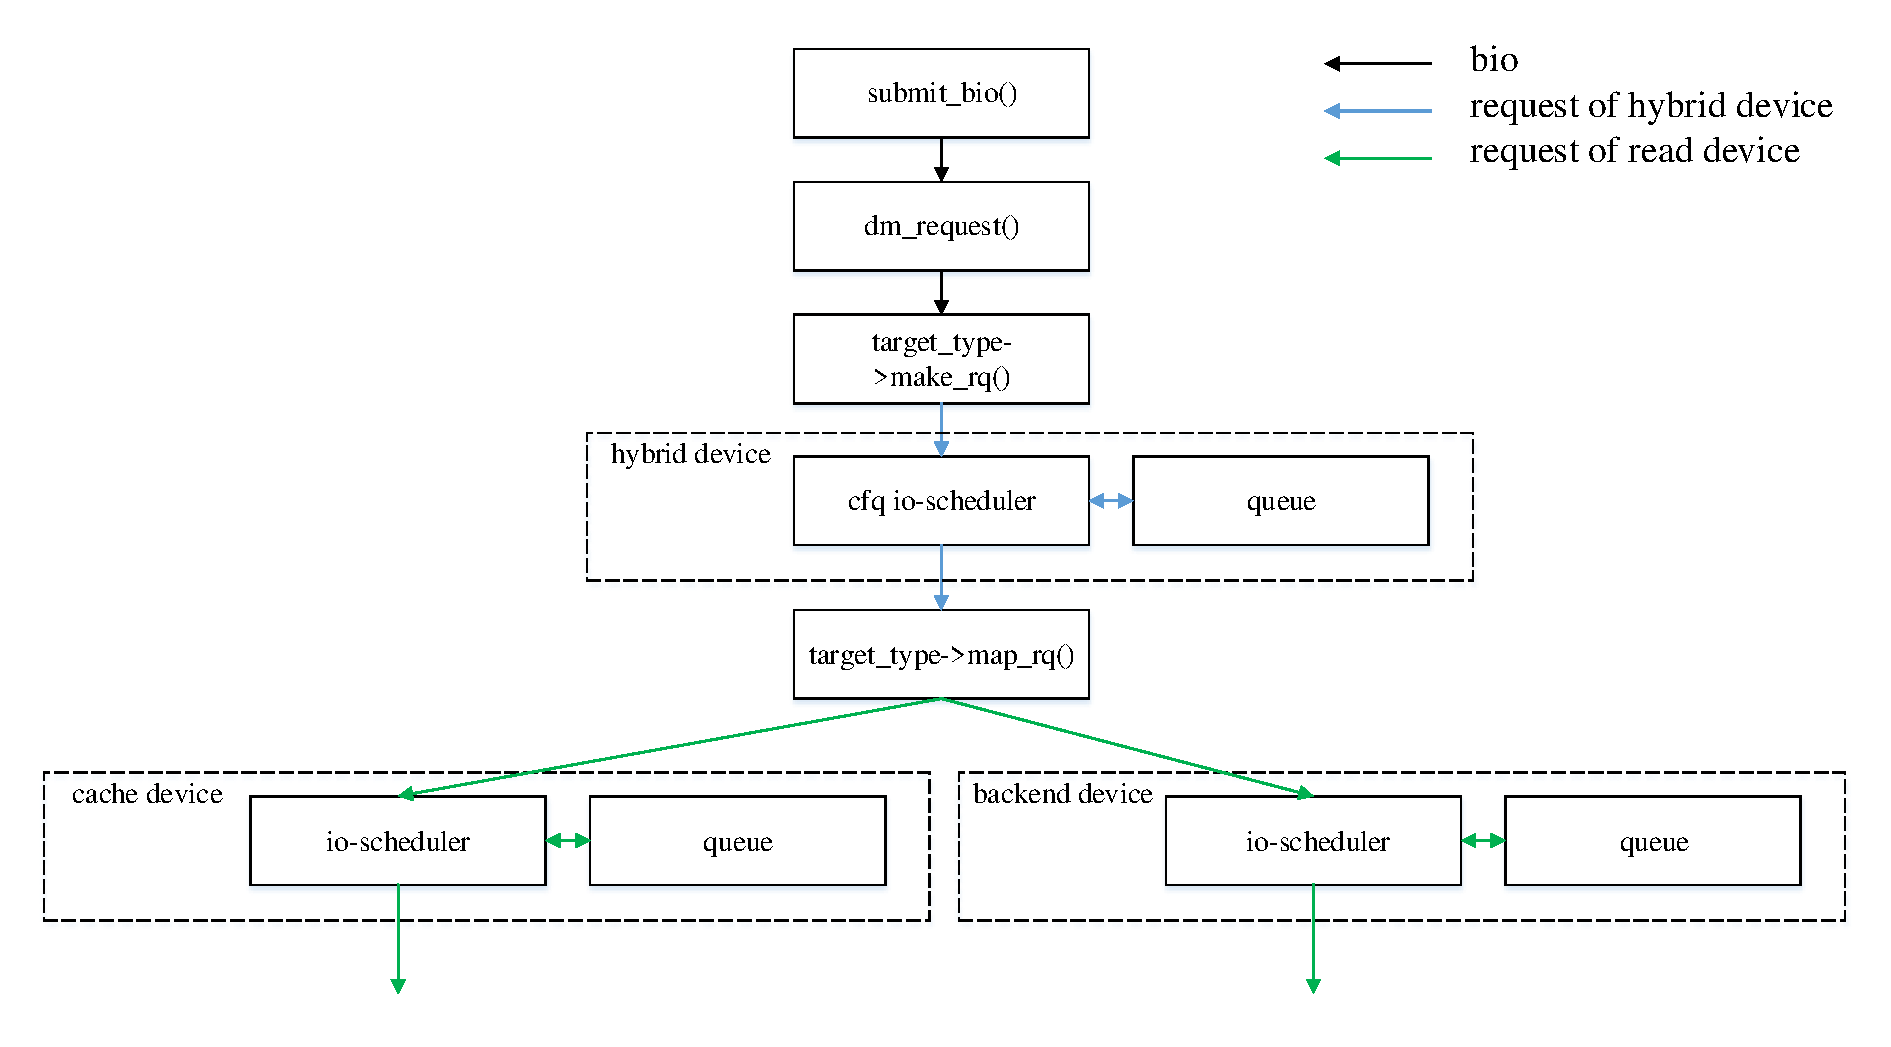
\includegraphics[width=\textwidth]{request_process.pdf}
    \bicaption[fig:request_process]{基于request的请求流程}{基于request的请求流程}{Fig}{request process in request-based system}
\end{figure}


\section{本章小结}

本章介绍了系统在实现中需要的预备知识以及具体的实现方法。预备知识主要介绍了Linux存储层次、bio和Device Mapper。具体的实现方法主要介绍了多缓存设备对多后台设备的实现以及按照进程的权限分配不同进程的I/O带宽的实现。